
\chapter{Reihen}
\setcounter{section}{13}
\setcounter{subsection}{0}
\setcounter{subsubsection}{-1}
\setcounter{secnumdepth}{4}
\subsection{Reihen}
\href{https://youtu.be/-YXCVGfMCcQ}{Video 01}\\
Eine (unendliche) Reihe hat die Form:\\
\begin{align*}
a_0+a_1+\ldots=\sum\limits_{k=0}^{\infty}a_k\;\;\text{mit }\;\;a_k\in\mathbb{R}\;\;\text{ für alle}\;\;k\in\mathbb{N}
\end{align*}
Dazu definieren wie die $ n-\text{te } $ Partialsumme:\\
\begin{align*}
\mathrm{S}_n:=\sum\limits_{k=0}^{n}a_k
\end{align*}
Die unendliche Reihe $ \sum\limits_{k=0}^{\infty}a_k $ heißt konvergent, wenn der Grenzwert von:\\
\begin{align*}
\lim\limits_ {n\to\infty}\mathrm{S}_n=\sum\limits_{k=0}^{\infty}a_k
\end{align*}
existiert.\\
\\
Bevor man eine Reihe bilden kann benötigt man eine Folge $ (a_k)_{\mathbb{N}} $. Nun summiert man die Folgeglieder auf und bildet die Partialsumme.\\
\begin{align*}
&\mathrm{S}_0=a_0=\sum\limits_{k=0}^{0}a_k\\
&\mathrm{S}_1=a_0+a_1=\sum\limits_{k=1}^{1}a_k\\
&\mathrm{S}_2=a_0+a_1+a_2=\sum\limits_{k=1}^{2}a_k\\
&\mathrm{S}_n=a_0+a_1+a_2+\ldots+a_n=\sum\limits_{k=0}^{n}a_k
\end{align*}
Konvergiert nun die Reihe für $ n\rightarrow\infty $, so existiert ein  Grenzwert $ \sum\limits_{k=0}^{\infty} a_k$. Die Reihe konvergiert dann, wenn die Folge konvergiert.\\
Durch $ \lim\limits_ {n\to\infty}\mathrm{S}_n=\sum\limits_{k=0}^{\infty} a_k$ übersetzen wir Begriffe wie Konvergenz, Divergenz und bestimmmte Divergenz.\\
\\
Beispiel:\\
\begin{align*}
\sum\limits_{k=0}^{\infty}a_k\;\;\text{mit }\;\;a_k=k\;\;\text{bzw. }\;\;\sum\limits_{k=0}^{\infty}k
\end{align*}
Es gilt (kann mittels Induktion bewiesen werden - Gaußsche Summenformel ):\\
\begin{align*}
\mathrm{S}_n=\sum\limits_{k=0}^{n}k=\frac{n(n+1)}{2}
\end{align*}
Für den Grenzwert: $ \lim\limits_ {n\to\infty} $ gilt:\\
\begin{align*}
\lim\limits_ {n\to\infty}\mathrm{S}_n=\sum\limits_{k=0}^{\infty}k=\lim\limits_ {k\to\infty}\frac{n(n+1)}{2}=\lim\limits_ {n\to\infty}\frac{n^2+n}{2}=\infty
\end{align*}
Die Partialsumme divergiert gegen das Unendliche.\\
\newpage
\noindent
\subsubsection{Beispiel zum Thema Reihen}
\href{https://youtu.be/hroOOlHucwM}{Video 02}\\
Gegeben die Reihe:\\
\begin{align*}
\sum\limits_{k=2}^{\infty}\bigg(\frac{1}{k-1}-\frac{1}{k}\bigg)
\end{align*}
Bestimme den Grenzwert $\lim\limits_ {n\to\infty} \mathrm{S}_n $:
\begin{align*}
\mathrm{S}_n=\sum\limits_{k=2}^{n}\bigg(\frac{1}{k-1}-\frac{1}{k}\bigg)&=\bigg(1-\frac{1}{2}\bigg)+\bigg(\frac{1}{2}-\frac{1}{3}\bigg)+\bigg(\frac{1}{3}-\frac{1}{4}\bigg)+\ldots+\bigg(\frac{1}{n-1}-\frac{1}{n}\bigg)\\
&=1\underbrace {-\frac{1}{2}+\frac{1}{2}}_{=0}\underbrace {-\frac{1}{3}+\frac{1}{3}}_{=0}\underbrace {-\frac{1}{4}+.}_{=0}\ldots\underbrace {.\bigg(\frac{1}{n-1}}_{=0}-\frac{1}{n}\bigg)\\
&=1-\frac{1}{n}\\
\lim\limits_ {n\to\infty}\mathrm{S}_n&=\lim\limits_ {n\to\infty}\bigg(1-\frac{1}{n}\bigg)=1-0=1\\
\end{align*}
\subsection{Gometrische Reihe}
\href{https://youtu.be/nmtUHgdMWXs}{Video 03}\\
\begin{center}
	\fbox{\parbox  {45mm} {Sei $ q\in\mathbb{R} $. Dann heißt\\$ \sum\limits_{k=0}^{\infty}q^k=1+q+q^2+\ldots $\\die geometrische Reihe}}	
\end{center}
Für die $ n- $te Partialsumme gilt:\\
\begin{align*}
\mathrm{S}_n =   \left\{ \begin{array}{rcl}
n+1 & \mbox{für} & q=1\\
\frac{1-q^2}{1-q}&\mbox{für}& q\neq1
\end{array}\right.
\end{align*}
Untersuchung der Konvergenz der geometrischen Reihe in Abängigkeit von $ q $.\\
\underline{Für $ q=1 $ gilt:}\\
\begin{quote}
	\begin{align*}
	\lim\limits_ {n\to\infty}\mathrm{S}_n=\lim\limits_ {n\to\infty}(n+1)=\infty
	\end{align*}
\end{quote}
\newpage
\noindent
\underline{Für $ q\neq 1 $ gilt:}\\
\begin{quote}
	1. Fall: $ q>1 $\\
	\begin{quote}
		\begin{align*}
		&\lim\limits_ {n\to\infty}\mathrm{S}_n=\lim\limits_ {n\to\infty}\bigg(\frac{1-q^{n+1}}{1-q}\bigg)\\
		\end{align*}
		
		\begin{align*}
		&\text{Es gilt für den Zähler: }\\
		&\lim\limits_ {n\to\infty}1-q^{n+1}=-\infty\\
		&\text{Es gilt für den Nenner: }\\
		&1-q<0\\
		&\Rightarrow \text{Der Bruch geht gegen}+\infty
		\end{align*}
		
	\end{quote}
	2. Fall: $ -1<q<1 $\\
	\begin{quote}
		\begin{align*}
		&\lim\limits_ {n\to\infty}\mathrm{S}_n=\lim\limits_ {n\to\infty}\bigg(\frac{1-q^{n+1}}{1-q}\bigg)\\
		\end{align*}
		\begin{align*}
		&\text{Es gilt für den Zähler: }\\
		&\lim\limits_ {n\to\infty}1-q^{n+1}=1\\
		&\text{Es gilt für den Nenner: }\\
		&1-q>0\\
		&\Rightarrow \lim\limits_ {n\to\infty}\biggl(\frac{1-q^{n+1}}{1-q}\biggr)=\frac{1}{1-q}
		\end{align*}
	\end{quote}
	3. Fall: $ q\leq -1 $\\
	\begin{quote}
		\begin{align*}
		&\lim\limits_ {n\to\infty}\mathrm{S}_n=\lim\limits_ {n\to\infty}\bigg(\frac{1-q^{n+1}}{1-q}\bigg)\\
		\end{align*}
		Es existiert kein Grenzwert, weil $ q^n $ für $ q\leq -1 $ alterniert.\\
		Diese Folge ist nicht konvergent.\\
	\end{quote}
\end{quote}
Fazit:\\
Für $ -1<q<1 $ oder $ |q| <1$ ist die geometrische Reihe konvergent.\\
\begin{center}
	\boxed{ \sum\limits_{k=0}^{\infty}q^k=\lim\limits_ {n\to\infty}\mathrm{S}_n=\frac{1}{1-q} }	
\end{center}
\subsubsection{Aufgabe zur geometrischen Reihe}
\href{https://youtu.be/FlwGJnrlD4c}{Video 04}\\
Zeige, dass die Summe: $ \sum\limits_{k=2}^{\infty}\frac{2^{k+1}}{5\cdot 3^k} $  konvergent ist und berechne den Grenzwert.\\
\begin{align*}
\sum\limits_{k=2}^{\infty}\underbrace {\frac{2^{k+1}}{5\cdot 3^k}}_{=a_k}
\end{align*}
\begin{align*}
a_k=\frac{2^{k+1}}{5\cdot 3^k}=\frac{2}{5}\cdot \frac{2^k}{3^k}=\frac{2}{5}\cdot \bigg(\frac{2}{3}\bigg)^k
\end{align*}
Dann gilt:\\
\begin{align*}
\sum\limits_{k=2}^{\infty}\frac{2^{k+1}}{5\cdot 3^k}=\sum\limits_{k=2}^{\infty}\frac{2}{5}\cdot \bigg(\frac{2}{3}\bigg)^k=\frac{2}{5}\sum\limits_{k=2}^{\infty}\bigg(\frac{2}{3}\bigg)^k
\end{align*}
Damit man die geometrische Reihe anwenden kann muss die Summe mit $ k=0 $ beginnen.\\
\begin{align*}
\frac{2}{5}\sum\limits_{k=2}^{\infty}\bigg(\frac{2}{3}\bigg)^k=\frac{2}{5}\sum\limits_{k=0}^{\infty}\bigg(\frac{2}{3}\bigg)^k-\frac{2}{5}\bigg(\frac{2}{3}\bigg)^0-\frac{2}{5}\bigg(\frac{2}{3}\bigg)^1=\frac{2}{5}\sum\limits_{k=0}^{\infty}\bigg(\frac{2}{3}\bigg)^k-\frac{2}{3}
\end{align*}
Mit der geometrischen Reihe gilt für $ |q|<1:\;\;\sum\limits_{k=0}^{\infty}q^k=\frac{1}{1-q} $:\\
\begin{align*}
\sum\limits_{k=2}^{\infty}\frac{2^{k+1}}{5\cdot 3^k}&=\frac{2}{5}\underbrace {\sum\limits_{k=0}^{\infty}\bigg(\frac{2}{3}\bigg)^k}_{=\frac{1}{1-q}}-\frac{2}{3}\\
&=\frac{2}{5}\bigg(\frac{1}{1-\frac{2}{3}}\bigg)-\frac{2}{3}\\
&=\frac{6}{5}-\frac{2}{3}=\frac{8}{15}
\end{align*}
Fazit:
\begin{align*}
\sum\limits_{k=2}^{\infty}\frac{2^{k+1}}{5\cdot 3^k}=\frac{8}{15} 
\end{align*}
\subsection{Rechenregeln für konvergente Reihen}
\href{https://youtu.be/Hs5s1w53hmI}{Video 05}\\
Seien $ \sum\limits_{k=0}^{\infty} a_k=\mathrm{A}$ und $ \sum\limits_{j=0}^{\infty}b_j=\mathrm{B} $ konvergierende Reihen.\\
Dann gilt:\\
\begin{align*}
\begin{array}{lll}
\text{(i) }&\sum\limits_{k=0}^{\infty}(a_k+b_k)=\sum\limits_{k=0}^{\infty}a_k+\sum\limits_{j=0}^{\infty}b_j=\mathrm{A}+\mathrm{B}\\[15pt]%Zeilenvorschub
\text{(ii) }&\sum\limits_{k=0}^{\infty}(\mathrm{C}\cdot a_k)=\mathrm{C}\sum\limits_{k=0}^{\infty}a_k=\mathrm{C}\cdot\mathrm{A}\;\;\text{für }\mathrm{C}\in\mathbb{R}\;\;\text{beliebig }\\[15pt]
\text{(iii) }&\sum\limits_{k=0}^{\infty}a_k\cdot\sum\limits_{k=0}^{\infty}b_k=\sum\limits_{k=0}^{\infty}c_k\;\;\text{, wobei } c_k=a_0\cdot b_k+a_1\cdot b_{k-1}+\ldots+a_k\cdot b_0\\
&\text{ gilt nur, wenn}\sum\limits_{k=0}^{\infty}c_k \;\;\text{konvergent ist. }
\end{array}
\end{align*}
Hinweis-Cauchy-Produkt: \\
Für $ n\in \mathbb{N} $ setzt man $ c_n:=\sum\limits_{k=0}^{n}a_k\cdot b_{n-k} $, so kann mann alle Summanten bestimmen.\\
\begin{align*}
&c_n=\sum\limits_{k=0}^{n}a_k\cdot b_{n-k}\\
&c_0=a_0b_0\\
&c_1=a_0b_1+a_1b_0\\
&c_2=a_0b_2+a_1b_1+a_2b_0\\
&c_3=a_0b_3+a_1b_2+a_2b_1+a_3b_0\\
&\colon
\end{align*}
\subsubsection{Notwendiges Konvergenzkriterium für Reihen}
\href{https://youtu.be/l_l4p0D7qro}{Video 06}\\
Sei $ \sum\limits_{k=0}^{\infty}a_k $ konvergent gegen $ \mathrm{A} $.\\
Dann gilt:\\
\begin{align*}
\lim\limits_ {n\to\infty}\mathrm{S}_n=\mathrm{A}=\lim\limits_ {n\to\infty}\mathrm{S}_{n-1}
\end{align*}
Bemerkung:\\
Der Grenzwert z.B. von $ \lim\limits_ {n\to\infty}\frac{1}{n}= 0 $ und $ \lim\limits_ {n\to\infty}\frac{1}{n+1}=0 $.\\
\begin{align*}
&\mathrm{S}_n=\sum\limits_{k=0}^{n}a_k\\
&\lim\limits_ {n\to\infty}\mathrm{S}_n=\mathrm{A}=\lim\limits_ {n\to\infty}\mathrm{S}_{n-1}\\
&\Leftrightarrow \lim\limits_ {n\to\infty}(\mathrm{S}_n-\mathrm{S}_{n-1})=\mathrm{A}-\mathrm{A}=0\\
\end{align*}
\begin{align*}
\mathrm{S}_n-\mathrm{S}_{n-1}=\sum\limits_{k=0}^{n}a_k-\sum\limits_{k=0}^{n-1}a_k=a_n
\end{align*}
Bei der Differenz von $ \sum\limits_{k=0}^{n}a_k-\sum\limits_{k=0}^{n-1}a_k $ bleibt nur noch das Glied $ a_n $ über.\\
Also ist der Grenzwert von:\\
\begin{align*}
\lim\limits_ {n\to\infty}(\mathrm{S}_n-\mathrm{S}_{n-1})=\lim\limits_ {n\to\infty}a_n=0
\end{align*}
Fazit:\\
Wenn $ \sum\limits_{k=0}^{\infty}a_k $ ist konvergent $ \Rightarrow \lim\limits_ {n\to\infty}a_n=0$.\\
Wenn $ \lim\limits_ {n\to\infty}a_n\neq 0\Rightarrow\sum\limits_{k=0}^{\infty}a_k $ ist nicht konvergent.\\
\newpage
\noindent
Beispiel:\\
\begin{align*}
\sum\limits_{k=0}^{\infty}\frac{k+1}{k+2}
\end{align*}
Diese Reihe ist nicht konvergent wegen dem notwendigen Konvergenzkriterium:\\
\begin{align*}
\lim\limits_ {k\to\infty}a_k=\lim\limits_ {k\to\infty} \bigg(\frac{k+1}{k+2}\bigg)=\frac{k(1+\frac{1}{k})}{k(1+\frac{2}{k})}=1\neq 0
\end{align*}
Daraus folgt, dass die Reihe:$ \sum\limits_{k=0}^{\infty}\frac{k+1}{k+2}=1 $ divergiert.\\
Achtung:\\
Der Umkehrschluss gilt nicht. Ist die Reihe divergent dann muss die Folge auch nicht divergent sein.\\
Beispiel:\\
$ \sum\limits_{k=1}^{\infty}\frac{1}{k} $ ist divergent, aber der Grenzert von: $ \lim\limits_ {k\to\infty}\frac{1}{k}=0 $.\\
\subsubsection{Majorantenkriterium für Reihen}
\href{https://youtu.be/qShFeav_pYk}{Video 07}\\
Sei $ \sum\limits_{k=0}^{\infty}a_k $ und $ \sum\limits_{k=0}^{\infty}b_k $ gegeben.\\
Existiert ein $ k_o\in \mathbb{N} $, so dass gilt:\\
\begin{align*}
|a_k|\leq b_k\;\;\text{ für alle}\; k\geq k_o
\end{align*}
und ist $ \sum\limits_{k=0}^{\infty}b_k $ konvergent, dann ist auch $ \sum\limits_{k=0}^{\infty}a_k $ konvergent.\\
\\
Beispiel:\\
Ist die Reihe: $ \sum\limits_{k=0}^{\infty}\frac{1}{r^2}=a_k $ konvergent ?\\
Es gilt: Die Reihe: $ \sum\limits_{k=2}^{\infty}\frac{1}{k-1}-\frac{1}{k}=b_k $ ist konvergent.\\
Wir betrachten:\\
\begin{align*}
|a_k|=\frac{1}{k^2}=\frac{1}{k}\cdot\frac{1}{k}&<\frac{1}{(k-1)}\cdot\frac{1}{k}\;\;\text{für }\;k\geq 2\\
&<\frac{k-k+1}{k(k-1)}=\frac{k}{k(k-1)}+\frac{-k+1}{k(k-1)}=\frac{1}{k-1}+\frac{-1(k-1)}{k(k-1)}=\frac{1}{k-1}-\frac{1}{k}=b_k\\
|a_k|&<b_k
\end{align*}
Fazit:\\
Da $ |a_k|=\frac{1}{k^2}<\frac{1}{k-1}-\frac{1}{k}=b_k $ für $ k\geq2 $ und $ \sum\limits_{k=2}^{\infty}\frac{1}{k-1}-\frac{1}{k} $ konvergent ist folgt mit dem Majorantenkriterium:\\
\begin{align*}
\sum\limits_{k=0}^{\infty}\frac{1}{k^2}\;\;\text{ist konvergent. }\\
\end{align*}
\subsubsection{Quotientenkriterium für Reihen}
\href{https://youtu.be/6xdKQ09P7c4}{Video 08}\\
Sei $ \sum\limits_{k=0}^{\infty} a_k $ gegeben. Dann gilt:\\
\begin{align*}
\begin{array}{lll}
\text{(i) }&\sum\limits_{k=0}^{\infty}\big|\frac{a_{k+1}}{a_k}\big|<1\Rightarrow \sum\limits_{k=0}^{\infty}a_k \;\;\text{ist konvergnet }\\[15pt]%Zeilenvorschub
\text{(ii) }&\sum\limits_{k=0}^{\infty}\big|\frac{a_{k+1}}{a_k}\big|>1\Rightarrow \sum\limits_{k=0}^{\infty}a_k \;\;\text{ist divergent }\\[15pt]%Zeilenvorschub
\text{(iii) }&\sum\limits_{k=0}^{\infty}\big|\frac{a_{k+1}}{a_k}\big|=1\;\text{oder nicht existent, dann kann man keine Aussage machen! }\\[15pt]%Zeilenvorschub
\end{array}
\end{align*}
Beispiel: \\
\begin{align*}
\sum\limits_{k=0}^{\infty}\frac{k}{2^k}
\end{align*}
Betrachte:\\
\begin{align*}
\bigg|\frac{a_{k+1}}{a_k}\bigg|
\end{align*}
Denn Betrag kann man weglassen, weil Zähler und Nenner immer  positv werden.\\
\begin{align*}
\frac{a_{k+1}}{a_k}=\frac{\frac{k+1}{2^{k+1}}}{\frac{k}{2^k}}=\frac{(k+1)(2^k)}{(2^{k+1})(k)}
\end{align*}
Für $ k\neq 0 $ gilt dann:\\
\begin{align*}
\frac{a_{k+1}}{a_k}=\frac{(k+1)(2^k)}{(2^{k+1})(k)}=\frac{1}{2}\cdot\frac{k+1}{k}
\end{align*}
Für $ k\mapsto\infty $ gilt:\\
\begin{align*}
\lim\limits_ {k\to\infty}\frac{1}{2}\cdot\frac{k+1}{k}=\frac{1}{2}\cdot\frac{k(1+\frac{1}{k})}{k}=\frac{1}{2}
\end{align*}
Daraus folgt mit dem Quotientenkriterium:\\
\begin{align*}
\lim\limits_ {k\to\infty}\frac{a_{k+1}}{a_k}=\frac{(k+1)(2^k)}{(2^{k+1})(k)}=\frac{1}{2}<1\Rightarrow \;\;\text{Die Reihe ist konvergent. }
\end{align*}
\newpage
\noindent
\paragraph{Aufgabe zum Quotientenkriterium für Reihen}$  $\vspace*{3mm}\\
\href{https://youtu.be/Zp1q1k58Tqk}{Video 09}\\
Ist die Reihe $ \sum\limits_{k=1}^{\infty}\frac{(-1)^k(k+1)!}{2\cdot 4\cdot 6 \cdot\ldots \cdot 2k} $ konvergent?\\
Daraus folgt mit dem Quotientenkriterium mit $ a_k=\frac{(-1)^k(k+1)!}{2\cdot 4\cdot 6 \cdot\ldots \cdot 2k} $ :\\
\begin{align*}
\lim\limits_ {k\to\infty}\bigg|\frac{a_{k+1}}{a_k}\bigg|&=\Bigg|\frac{\frac{(-1)^{k+1}(k+2)!}{2\cdot 4\cdot 6\cdot\ldots\cdot 2(k+1)}}{\frac{(-1)^{k}(k+1)!}{2\cdot 4\cdot 6\cdot\ldots\cdot 2k}}\Bigg|\\
&=\frac{2\cdot 4\cdot 6\cdot\ldots\cdot2k(k+2)!}{2\cdot 4\cdot 6 \cdot\ldots \cdot 2(k+1)(k+1)!}\\
&=\frac{2\cdot 4\cdot 6\cdot\ldots\cdot2k(k+2)(k+1)!}{2\cdot 4\cdot 6 \cdot\ldots \cdot 2(k+1)(k+1)!}\\
&=\frac{2\cdot 4\cdot 6\cdot\ldots\cdot2k(k+2)}{2\cdot 4\cdot 6\cdot\ldots\cdot2(k+1)}\\
&=\frac{2\cdot 4\cdot 6\cdot\ldots\cdot2k(k+2)}{2\cdot 4\cdot 6\cdot\ldots\cdot (2k+2)}\text{\tiny vorletzter Faktor im Nenner ist $ 2k $ und der Letzte $ 2k+2 $}\\
&=\frac{2\cdot 4\cdot 6\cdot\ldots\cdot2k(k+2)}{2\cdot 4\cdot 6\cdot\ldots\cdot 2k\cdot(2k+2)}\\
&=\frac{(k+2)}{(2k+2)}\\
&=\frac{(k+2)}{2(k+1)}=\frac{1}{2}\cdot\frac{k(1+\frac{2}{k})}{k(1+\frac{1}{k})}=\frac{1}{2}<1
\end{align*}
Daraus folgt nach dem Quotientenkriterium, dass die Folge:\\
\begin{align*}
\sum\limits_{k=1}^{\infty}\frac{(-1)^k(k+1)!}{2\cdot 4\cdot 6 \cdot\ldots \cdot 2k}
\end{align*}
konvergent ist.\\
\newpage
\noindent
\subsubsection{Wurzelkriterium für Reihen}
\href{https://youtu.be/axTFmjV9WSA}{Video 10}\\
Sei $ \sum\limits_{k=0}^{\infty} a_k $ gegeben. Dann gilt:\\
\begin{align*}
\begin{array}{lll}
\text{(i) }&\lim\limits_ {k\to\infty}|\sqrt[k]{a_k}|=\lim\limits_ {k\to\infty}|a_k|^{\frac{1}{k}}<1\Rightarrow \sum\limits_{k=0}^{\infty}a_k\;\;\text{ist konvergent }\\[15pt]%Zeilenvorschub
\text{(ii) }&\lim\limits_ {k\to\infty}|\sqrt[k]{a_k}|=\lim\limits_ {k\to\infty}|a_k|^{\frac{1}{k}}\geq 1\Rightarrow \sum\limits_{k=0}^{\infty}a_k\;\;\text{ist für unendlich viele $ k $ divergent}\\[15pt]%Zeilenvorschub
\end{array}
\end{align*}
Beispiel:\\
Ist die Reihe: $ \sum\limits_{k=0}^{\infty}\big(-\frac{1}{2^k}\big)^k $ konvergent ?\\
Daraus folgt mit dem Wurzelkriterium mit $ a_k=\big(-\frac{1}{2^k}\big)^k $ :\\
\begin{align*}
\lim\limits_ {k=0\to\infty}|\sqrt[k]{a_k}|=\bigg|\sqrt[k]{\bigg(-\frac{1}{2^k}\bigg)^k }\bigg|=\bigg|\bigg(\frac{(-1)^k}{2^{k\cdot k}}\bigg)\bigg|^{\frac{1}{k}}=\bigg(\frac{1}{2^{k^2}}\bigg)^{\frac{1}{k}}=\frac{1}{2^k}=0<1
\end{align*}
Daraus folgt nach dem Wurzelkriterium, dass die Folge:\\
\begin{align*}
\sum\limits_{k=0}^{\infty}\bigg(-\frac{1}{2^k}\bigg)^k
\end{align*}
konvergent ist.\\
\paragraph{Aufgabe zum Wurzelkriterium für Reihen}$  $\vspace*{3mm}\\
\href{https://youtu.be/Z95Uw9OgMck}{Video 11}\\
Zeige, dass diese Folge konvergent ist:\\
\begin{align*}
\sum\limits_{k=0}^{\infty}\frac{k}{3^k}
\end{align*}
Def.:\\
\begin{align*}
a_k=\frac{k}{3^k}
\end{align*}
Berechne:\\
\begin{align*}
\sqrt[k]{|a_k|}&=\sqrt[k]{\frac{k}{3^k}}=\frac{\sqrt[k]{k}}{\sqrt[k]{3^k}}=\frac{\sqrt[k]{k}}{3}
\end{align*}
NR.:\\
\begin{align*}
\sqrt[k]{3^k}=\big(3^k\big)^{\frac{1}{k}}=3^{k\cdot\frac{1}{k}}=3^1=1
\end{align*}
Berechne den Grenzwert:\\
\begin{align*}
\lim\limits_ {k\to\infty}\frac{1}{3}\sqrt[k]{k}=\lim\limits_ {k\to\infty}\frac{1}{3}k^{\frac{1}{k}}=\frac{1}{3}\lim\limits_ {k\to\infty}\mathrm{e}^{\ln(k)\cdot\frac{1}{k}}
\end{align*}
Da die Funktion $ \mathrm{e}^x $ stetig ist, kann man den Grenzwert in die \glqq Potenz\grqq  ziehen.\\
\begin{align*}
\lim\limits_ {k\to\infty}\frac{1}{3}\sqrt[k]{k}=\frac{1}{3}\mathrm{e}^{\lim\limits_ {k\to\infty}\ln(k)\cdot\frac{1}{k}}
\end{align*}
Für den Grenzwert von $\lim\limits_ {k\to\infty}\ln(k)\cdot\frac{1}{k} $ gilt:\\
\begin{align*}
\lim\limits_ {k\to\infty}\frac{\ln(k)}{k}=0
\end{align*}
Bemerkung:\\
Der Logarithmus $ \ln(k) $wächst langsamer als der Bruch $ \frac{1}{k} $, deswegen geht der Grenzwert gegen Null.\\
Nun gilt:\\
\begin{align*}
&\lim\limits_ {k\to\infty}\frac{1}{3}\sqrt[k]{k}=\frac{1}{3}\mathrm{e}^{\lim\limits_ {k\to\infty}\ln(k)\frac{1}{k}}=\frac{1}{3}\mathrm{e}^0=\frac{1}{3}<1\\
&\Rightarrow \sum\limits_{k=0}^{\infty}\frac{k}{3^k}\;\;\text{konvergiert}
\end{align*}
\subsubsection{Das Leibnizkriterium}
\href{https://youtu.be/BM329RZgnwg}{Video 12}\\
Eine Reihe $ \sum\limits_{k=0}^{\infty} a_k$ heißt alternierent, wenn gilt: 
\begin{align*}
a_k\cdot a_{k+1}<0
\end{align*}
Die Summanten haben hintereinander verschiedene Vorzeichen.\\
\begin{align*}
\overset{-}{a_0}+\overset{+}{a_0}+\overset{-}{a_0}+\overset{+}{a_0}+\\
\overset{+}{a_0}+\overset{-}{a_0}+\overset{+}{a_0}+\overset{-}{a_0}+\\
\end{align*}
Beispiel:\\
\begin{align*}
\sum\limits_{k=0}^{\infty}(-1)^k=1-1+1-1\pm\ldots=0
\end{align*}
Die Summe wird $ 0 $, wenn man folgende Summanten addiert:\\
\begin{align*}
\sum\limits_{k=0}^{\infty}(-1)^k=\underbrace {1-1}_{=0}+\underbrace {1-1}_{=0}+\underbrace {1-1}_{=0}+\underbrace {1-1}_{=0}\pm\ldots=0
\end{align*}
Die Summe wird $ 1 $, wenn man folgende Summanten addiert:\\
\begin{align*}
\sum\limits_{k=0}^{\infty}(-1)^k=1\underbrace {-1+1}_{=0}\underbrace {-1+1}_{=0}\underbrace {-1+1}_{=0}\underbrace {-1+1}_{=0}\pm\ldots=1
\end{align*}
Die Summe wird $ 20 $, wenn man folgende Summanten addiert:\\
\begin{align*}
\sum\limits_{k=0}^{\infty}(-1)^k=\underbrace {1+\ldots +1}_{20\text{\tiny mal }}\underbrace {+1-1+1-1+1}_{=0}\pm\ldots=20\
\end{align*}
\\
\underline{Leibnizkriterium:}\\
Sei $ \sum\limits_{k=0}^{\infty}a_k $ eine alternierende Reihe\\ und ist $ \big(|a_k|\big)_k $ eine monoton fallende Nullfolge, dann konvergiert $ \sum\limits_{k=0}^{\infty}a_k $.
\\
Bemerkung:\\
Da kein Grenzwert bei der Reihe $\sum\limits_{k=0}^{\infty} (-1)^k  $ existiert und dies ist ja ein notwendiges Kriterium für eine Konvergenz ist divergiert die Reihe $ \sum\limits_{k=0}^{\infty} (-1)^k$.\\
\\
Betrachte die Reihe:\\
\begin{align*}
\sum\limits_{k=1}^{\infty}(-1)^k\frac{1}{k}
\end{align*}
\begin{align*}
a_k=(-1)^k\frac{1}{k}
\end{align*}
Wegen:
\begin{align*}
\big(|a_k|\big)_{k\in \mathbb{N}}=\bigg(\frac{1}{k}\bigg)_{k\in\mathbb{N}\setminus\{0\}}
\end{align*}
Bemerkung:\\
\begin{align*}
\bigg|(-1)^k\cdot\frac{1}{k}\bigg|=\frac{1}{k}
\end{align*}
Da $\big(\frac{1}{k}\big)_{k\in\mathbb{N}\setminus\{0\}}  $ eine streng monoton fallende Nullfolge ist, folgt mit dem Leinbnizkriterium, dass die Folge $ \sum\limits_{k=1}^{\infty}(-1)^k\frac{1}{k} $ konvergent ist.\\
Bemerkung:
Die Reihe $ \sum\limits_{k=1}^{\infty}\frac{1}{k} $ ist divergent.\\
\newpage
\noindent
\paragraph{Aufgabe zum Leibnizkriterium}$  $\vspace*{3mm}\\
\href{https://youtu.be/95O_7qUchvg}{Video 13}\\
Zeige, dass diese Folge konvergent ist.\\
\begin{align*}
\sum\limits_{k=2}^{\infty}(-1)^k\cdot \bigg(\frac{1}{k-1}-\frac{1}{k+2}\bigg)
\end{align*}
Mit dem Leibnizkriterium ist zu zeigen, dass $ \big(|a_k|\big)_{k\in \mathbb{N}_{k\geq 2}} $ eine monoton fallende Nullfolge ist.\\
$ |q_k| $ ist bei dieser Reihe:\\
\begin{align*}
|a_k|&=\bigg|(-1)^k\cdot \bigg(\frac{1}{k-1}-\frac{1}{k+2}\bigg) \bigg|\\
&=\bigg|(-1)^k\cdot\frac{k+2-(k-1)}{(k-1)(k+2)}\bigg|\\
|a_k|&=\bigg|(-1)^k\cdot\frac{3}{(k-1)(k+2)}\bigg|\\
\end{align*}
\underline{I. Monotonie}\\
Zz.: $ |a_k|\geq |a_{k+1}| $ für $ k\in \mathbb{N}_{k\geq 2} $\\
\begin{align*}
\Rightarrow &|a_k|-|a_{k+1}|\geq 0\\
&\bigg|(-1)^k\cdot\frac{3}{(k-1)(k+2)}\bigg|-\bigg|(-1)^k\cdot\frac{1}{(k+1-1)(k+1+2)}\bigg|\geq 0\\
&\frac{3}{(k-1)(k+2)}-\frac{1}{k(k+3)}\geq 0\\
&\frac{3k(k+3)-3(k-1)(k+2)}{(k-1)(k+2)k(k+3)}\geq 0\\
&\frac{3k^2+9k-3(k^2+k-2)}{(k-1)(k+2)k(k+3)}\geq 0\\
&\frac{3k^2+9k-3k^2-3k+6}{(k-1)(k+2)k(k+3)}\geq 0\\
&\frac{6k+6}{(k-1)(k+2)k(k+3)}\geq 0\\
\end{align*}
Da der Zähler immer größer Null ist:\\
\begin{align*}
6k+6>0
\end{align*}
Und der Nenner immer größer Null ist:\\
\begin{align*}
(k-1)(k+2)k(k+3)>0
\end{align*}
Ist der Bruch immer größer Null.
Daraus folgt: $ \big(|a_k| \big)_{k\in \mathbb{N}_{k\geq 2}}>0\Rightarrow |a_k|$ ist monoton fallend.\\
\\
\underline{II. Nullfolge:}\\
\begin{align*}
\lim\limits_ {k\to\infty}|a_k|=\lim\limits_ {k\to\infty}\frac{3}{(k-1)(k+2)}=\lim\limits_ {k\to\infty}\frac{1}{k^2+k+2}=0
\end{align*}
Fazit: Wegen I.und II. ist $ \big(|a_k|\big)_k{k\in\mathbb{N}_{k\geq2}} $ eine monoton fallende Nullfolge.\\

\begin{align*}
\overset{(Leibniz)}{\Rightarrow} \sum\limits_{k=2}^{\infty} (-1)^k\cdot\bigg(\frac{1}{k-1}-\frac{1}{k+2}\bigg)\;\;\text{ist konvergent. }
\end{align*}
\subsubsection{Das Reihen-Integral-Kriterium}
\href{https://youtu.be/x1s0KUSIwaQ}{Video 14}\\
Sei $ f:[n,\infty[ \;\mapsto \mathbb{R}$ eine monoton fallende Funktion mit $ f(x) \geq 0$ für $ x\in [n,\infty[ \;$.\\
\begin{align*}
\int\limits_{n}^{\infty} f(x)dx\;\;\text{existiert }\Leftrightarrow \sum\limits_{k=n}^{\infty}f(k)\;\;\text{konvergiert }
\end{align*}
\begin{center}
	
	Wenn dieses Integral $ f(x) $ existiert,\\	
	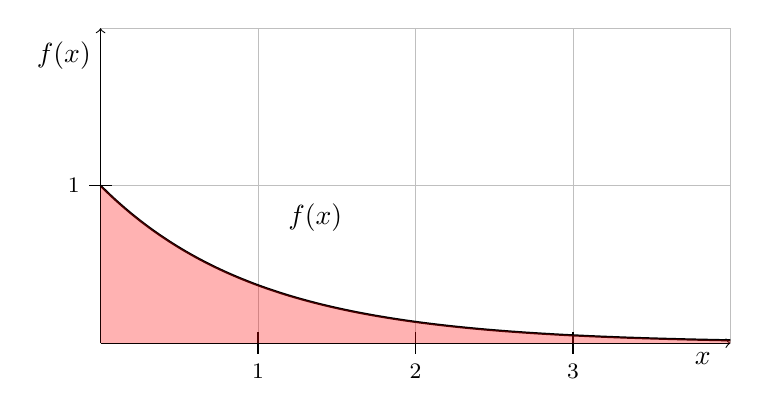
\begin{tikzpicture}[xscale=2, yscale=2]
	
	% Gitternetzlinien
	\draw[xstep=1cm, ystep=1cm, very thin, color=lightgray] (0,2) grid (4,0);
	% x-Achse
	\draw[->] (0,0) -- (4,0) node[below,xshift=-1em] {$x$}; 
	%Zahlen auf x-Achse
	%\foreach \x in {-1,...,-1}
	%\draw[shift={(\x,0)},color=black] (0pt,2pt) -- (0pt,-2pt) node[below] {\footnotesize $\x$};
	\foreach \x in {1,...,3}
	\draw[shift={(\x,0)},color=black] (0pt,2pt) -- (0pt,-2pt) node[below] {\footnotesize $\x$};
	% y-Achse 
	\draw[->] (0,0) -- (0,2) node[left,yshift=-1em] {$f(x)$};%node[above left]
	%Zahlen auf y-Achse
	%\foreach \y in {0,...,-1}
	%\draw[shift={(0,\y)},color=black] (2pt,0pt) -- (-2pt,0pt) node[left] {\footnotesize $\y$};
	\foreach \y in {1,...,1}
	\draw[shift={(0,\y)},color=black] (2pt,0pt) -- (-2pt,0pt) node[left] {\footnotesize $\y$};
	%Ursprung
	%\draw[color=black] (0pt,-10pt) node[right] {\footnotesize $0$};
	
	\draw[thick,color=black] plot[samples=200, domain=0:4] 
	(\x,{e^(-\x)}) node[below, xshift=-15em,yshift=53] {$f(x)$};
	%\draw[color=black] (.5,0.2) node[right] {\footnotesize $\mathrm{A}=1$};
	\fill[color =red,fill opacity=0.3] plot[domain=0:4] (\x,{e^(-\x) })% 
	-- plot[domain=4:0] (\x,{0});% 
	
	
	
	\end{tikzpicture}\\
\end{center}
\begin{center}
	dann existiert auch die Folge $ \sum\limits_{k=n}^{\infty}f(k) $.
	
	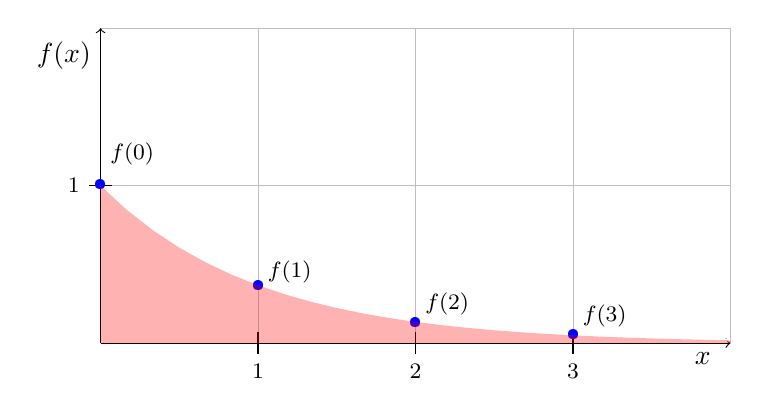
\begin{tikzpicture}[xscale=2, yscale=2]
	
	% Gitternetzlinien
	\draw[xstep=1cm, ystep=1cm, very thin, color=lightgray] (0,2) grid (4,0);
	% x-Achse
	\draw[->] (0,0) -- (4,0) node[below,xshift=-1em] {$x$}; 
	%Zahlen auf x-Achse
	%\foreach \x in {-1,...,-1}
	%\draw[shift={(\x,0)},color=black] (0pt,2pt) -- (0pt,-2pt) node[below] {\footnotesize $\x$};
	\foreach \x in {1,...,3}
	\draw[shift={(\x,0)},color=black] (0pt,2pt) -- (0pt,-2pt) node[below] {\footnotesize $\x$};
	% y-Achse 
	\draw[->] (0,0) -- (0,2) node[left,yshift=-1em] {$f(x)$};%node[above left]
	%Zahlen auf y-Achse
	%\foreach \y in {0,...,-1}
	%\draw[shift={(0,\y)},color=black] (2pt,0pt) -- (-2pt,0pt) node[left] {\footnotesize $\y$};
	\foreach \y in {1,...,1}
	\draw[shift={(0,\y)},color=black] (2pt,0pt) -- (-2pt,0pt) node[left] {\footnotesize $\y$};
	%Ursprung
	%\draw[color=black] (0pt,-10pt) node[right] {\footnotesize $0$};
	
	\draw[thick,color=white] plot[samples=200, domain=0:4] 
	(\x,{e^(-\x)}) node[below, xshift=-15em,yshift=53] {$f(x)$};
	\draw[color=black] (1,0.45) node[right] {\footnotesize $f(1)$};
	\draw[color=black] (0,1.2) node[right] {\footnotesize $f(0)$};
	\draw[color=black] (2,0.25) node[right] {\footnotesize $f(2)$};
	\draw[color=black] (3,0.17) node[right] {\footnotesize $f(3)$};
	\draw[color=blue] (1,0.36) node {\textbullet};
	\draw[color=blue] (2,0.125) node {\textbullet};
	\draw[color=blue] (3,0.049) node {\textbullet};
	\draw[color=blue] (0,1) node {\textbullet};
	\fill[color =red,fill opacity=0.3] plot[domain=0:4] (\x,{e^(-\x) })% 
	-- plot[domain=4:0] (\x,{0});% 
	
	
	
	\end{tikzpicture}\\
\end{center}
\paragraph{Aufgabe zum Reihen-Integral-Kriterium}$  $\vspace*{3mm}\\
\href{https://youtu.be/x0s61IXjBKI}{Video 15}\\
Für welches $ \alpha\in\mathbb{R} $ konvergiert die Reihe $ \sum\limits_{k=1}^{\infty}\frac{1}{k^{\alpha}} $ ?\\
\renewcommand{\baselinestretch}{1.0}\normalsize
Es gilt:\\
\begin{align*}
\sum\limits_{k=1}^{\infty}\frac{1}{k^{\alpha}}\;\;\text{konvergiert }\Leftrightarrow\int\limits_{1}^{\infty}\frac{1}{x^{\alpha}} dx\;\;\text{existiert }
\end{align*}
\underline{1.Fall: $ \alpha=1 $}\\
\begin{align*}
&\int\limits_{1}^{\infty} \frac{1}{x}=\lim\limits_ {t\to\infty}\big[\ln(x)\big]_1^t=\lim\limits_ {t\to\infty}\ln(t)=\infty\\
&\Rightarrow \sum\limits_{k=1}^{\infty}\frac{1}{k}\;\;\text{divergiert }
\end{align*}
Bemerkung:\\
\begin{align*}
\sum\limits_{k=1}^{\infty}(-1)^k\frac{1}{k}\;\;\text{konvergiert }
\end{align*}
\underline{2.Fall:$ \alpha\neq 1 $}\\
\begin{align*}
\int\limits_{1}^{\infty} \frac{1}{x^{\alpha}}&=\lim\limits_ {t\to\infty}\int\limits_{1}^{t} x^{-\alpha}\\
&=\lim\limits_ {t\to\infty}\bigg|\frac{1}{1-\alpha}x^{1-\alpha}\bigg|_1^t\\
&=\lim\limits_ {t\to\infty}\bigg(\frac{1}{1-\alpha}t^{1-\alpha}-\frac{1}{1-\alpha}\bigg)
\end{align*}
\begin{quote}
	(i)\; wenn $ 1-\alpha>0 \Leftrightarrow\;\;\text{divergent }$\\
	(ii) wenn $ 1-\alpha<0 $
	\begin{quote}
		Es gilt für $ t^{1-\alpha} $ :\\
		Für $ \tilde{\alpha}=1-\alpha< 0\rightarrow \lim\limits_ {t\to\infty}\frac{1}{t^{\tilde{\alpha}}}=0$
	\end{quote}
	
	\begin{align*}
	&\frac{1}{1-\alpha}t^{1-\alpha}\;\;
	&\text{konvergiert gegen Null und der Grenzwert geht gegen } -\frac{1}{1-\alpha}=\frac{1}{\alpha-1}
	\end{align*}
\end{quote}
Fazit: Für $ \alpha>1 $ konvergiert $ \sum\limits_{k=1}^{\infty}\frac{1}{k^{\alpha}} $
